%  LaTeX support: latex@mdpi.com
%  In case you need support, please attach all files that are necessary for compiling as well as the log file, and specify the details of your LaTeX setup (which operating system and LaTeX version / tools you are using).

%=================================================================
\documentclass[genes, moreauthors]{Definitions/mdpi}

% If you would like to post an early version of this manuscript as a preprint, you may use preprint as the journal and change 'submit' to 'accept'. The document class line would be, e.g., \documentclass{mdpi}. This is especially recommended for submission to arXiv, where line numbers should be removed before posting. For preprints.org, the editorial staff will make this change immediately prior to posting.

%--------------------
% Class Options:
%--------------------
%----------
% journal
%----------
% Choose between the following MDPI journals:
% acoustics, actuators, addictions, admsci, aerospace, agriculture, agriengineering, agronomy, algorithms, animals, antibiotics, antibodies, antioxidants, applsci, arts, asc, asi, atmosphere, atoms, axioms, batteries, bdcc, behavsci , beverages, bioengineering, biology, biomedicines, biomimetics, biomolecules, biosensors, brainsci , buildings, cancers, carbon , catalysts, cells, ceramics, challenges, chemengineering, chemistry, chemosensors, children, cleantechnol, climate, clockssleep, cmd, coatings, colloids, computation, computers, condensedmatter, cosmetics, cryptography, crystals, dairy, data, dentistry, designs , diagnostics, diseases, diversity, drones, econometrics, economies, education, electrochem, electronics, energies, entropy, environments, epigenomes, est, fermentation, fibers, fire, fishes, fluids, foods, forecasting, forests, fractalfract, futureinternet, futurephys, galaxies, games, gastrointestdisord, gels, genealogy, genes, geohazards, geosciences, geriatrics, hazardousmatters, healthcare, heritage, highthroughput, horticulturae, humanities, hydrology, ijerph, ijfs, ijgi, ijms, ijns, ijtpp, informatics, information, infrastructures, inorganics, insects, instruments, inventions, iot, j, jcdd, jcm, jcp, jcs, jdb, jfb, jfmk, jimaging, jintelligence, jlpea, jmmp, jmse, jnt, jof, joitmc, jpm, jrfm, jsan, land, languages, laws, life, literature, logistics, lubricants, machines, magnetochemistry, make, marinedrugs, materials, mathematics, mca, medicina, medicines, medsci, membranes, metabolites, metals, microarrays, micromachines, microorganisms, minerals, modelling, molbank, molecules, mps, mti, nanomaterials, ncrna, neuroglia, nitrogen, notspecified, nutrients, ohbm, particles, pathogens, pharmaceuticals, pharmaceutics, pharmacy, philosophies, photonics, physics, plants, plasma, polymers, polysaccharides, preprints , proceedings, processes, proteomes, psych, publications, quantumrep, quaternary, qubs, reactions, recycling, religions, remotesensing, reports, resources, risks, robotics, safety, sci, scipharm, sensors, separations, sexes, signals, sinusitis, smartcities, sna, societies, socsci, soilsystems, sports, standards, stats, surfaces, surgeries, sustainability, symmetry, systems, technologies, test, toxics, toxins, tropicalmed, universe, urbansci, vaccines, vehicles, vetsci, vibration, viruses, vision, water, wem, wevj

%---------
% article
%---------
% The default type of manuscript is "article", but can be replaced by:
% abstract, addendum, article, benchmark, book, bookreview, briefreport, casereport, changes, comment, commentary, communication, conceptpaper, conferenceproceedings, correction, conferencereport, expressionofconcern, extendedabstract, meetingreport, creative, datadescriptor, discussion, editorial, essay, erratum, hypothesis, interestingimages, letter, meetingreport, newbookreceived, obituary, opinion, projectreport, reply, retraction, review, perspective, protocol, shortnote, supfile, technicalnote, viewpoint
% supfile = supplementary materials

%----------
% submit
%----------
% The class option "submit" will be changed to "accept" by the Editorial Office when the paper is accepted. This will only make changes to the frontpage (e.g., the logo of the journal will get visible), the headings, and the copyright information. Also, line numbering will be removed. Journal info and pagination for accepted papers will also be assigned by the Editorial Office.

%------------------
% moreauthors
%------------------
% If there is only one author the class option oneauthor should be used. Otherwise use the class option moreauthors.

%---------
% pdftex
%---------
% The option pdftex is for use with pdfLaTeX. If eps figures are used, remove the option pdftex and use LaTeX and dvi2pdf.

%=================================================================
\firstpage{1}
\makeatletter
\setcounter{page}{\@firstpage}
\makeatother
\pubvolume{xx}
\issuenum{1}
\articlenumber{5}
\pubyear{2019}
\copyrightyear{2019}
%\externaleditor{Academic Editor: name}
\history{Received: date; Accepted: date; Published: date}
%\updates{yes} % If there is an update available, un-comment this line

%% MDPI internal command: uncomment if new journal that already uses continuous page numbers
%\continuouspages{yes}

%------------------------------------------------------------------
% The following line should be uncommented if the LaTeX file is uploaded to arXiv.org
%\pdfoutput=1

%=================================================================
% Add packages and commands here. The following packages are loaded in our
%class file: fontenc, calc, indentfirst, fancyhdr, graphicx, lastpage, ifthen,
%lineno, float, amsmath, setspace, enumitem, mathpazo, booktabs, titlesec,
%etoolbox, amsthm, hyphenat, natbib, hyperref, footmisc, geometry, caption, url,
%mdframed, tabto, soul, multirow, microtype, tikz

%=================================================================

%% Please use the following mathematics environments: Theorem, Lemma,
%Corollary, Proposition, Characterization, Property, Problem, Example,
%ExamplesandDefinitions, Hypothesis, Remark, Definition
%% For proofs, please use the proof environment (the amsthm package is loaded by the MDPI class).

%=================================================================
% Full title of the paper (Capitalized)
\Title{NCBI's Virus Discovery Hackathon: Engaging Research Communities to Identify Cloud Infrastructure Requirements}

% Author Orchid ID: enter ID or remove command
\newcommand{\orcidauthorA}{0000-0000-000-000X} % Add \orcidA{} behind the author's name
%\newcommand{\orcidauthorB}{0000-0000-000-000X} % Add \orcidB{} behind the author's name

% Authors, for the paper (add full first names)
\Author{Firstname Lastname $^{1,\dagger,\ddagger}$\orcidA{}, Firstname Lastname $^{1,\ddagger}$ and Firstname Lastname $^{2,}$*}

% Authors, for metadata in PDF
\AuthorNames{Firstname Lastname, Firstname Lastname and Firstname Lastname}

% Affiliations / Addresses (Add  after \address if there is only one affiliation.)
\address{%
$^{1}$ \quad Affiliation 1; e-mail@e-mail.com\\
$^{2}$ \quad Affiliation 2; e-mail@e-mail.com}

% Contact information of the corresponding author
\corres{Correspondence: e-mail@e-mail.com; Tel.: (optional; include country code; if there are multiple corresponding authors, add author initials) +xx-xxxx-xxx-xxxx (F.L.)}

% Current address and/or shared authorship
\firstnote{Current address: Affiliation 3}
\secondnote{These authors contributed equally to this work.}
% The commands \thirdnote{} till \eighthnote{} are available for further notes

%\simplesumm{} % Simple summary

%\conference{} % An extended version of a conference paper

% Abstract (Do not insert blank lines, i.e. \\)
\abstract{A wealth of viral data sits untapped in publicly-available
metagenomic datasets when it might be extracted to create a usable index for
the virological research community. We hypothesized that work of this
complexity and scale could be done in a hackathon setting. Ten teams comprised
of over 40 participants from 6 countries, assembled to create a crowdsourced
pipeline of datasets in a three-day event on the San Diego State University
campus starting January 9$^{th}$, 2019. Contiguous assemblies (contigs) were
pre-assembled by National Center for Biotechnology Information (NCBI) staff
using the SKESA algorithm for a large sample of 141,000 metagenomic datasets
from the NCBI Sequence Read Archive (SRA).  During the Hackathon contigs were
aligned using BLAST against all known virus genomes, labeled with domains,
clustered, annotated, and assigned metadata. The work yielded valuable insights
into both SRA data and the cloud infrastructure required to support such
efforts, and the scientific findings will be extended during a follow-up
event.}

% Keywords
\keyword{keyword 1; keyword 2; keyword 3 (list three to ten pertinent keywords specific to the article, yet reasonably common within the subject discipline.)}

% The fields PACS, MSC, and JEL may be left empty or commented out if not applicable
%\PACS{J0101}
%\MSC{}
%\JEL{}


%\datasetlicense{license under which the data set is made available (CC0, CC-BY, CC-BY-SA, CC-BY-NC, etc.)}

%\setcounter{secnumdepth}{4}
%%%%%%%%%%%%%%%%%%%%%%%%%%%%%%%%%%%%%%%%%%
\begin{document}
  \section{Introduction}
  While advances in sequencing technology have greatly reduced the cost of
  whole genome sequencing \cite{Mardis2011}, it has given rise to new problems,
  especially related to data analysis and management. As the number of bases in
  the Sequence Read Archive \cite{Kodama2012} exceeds 33 petabases (June 2019),
  the difficulty to navigate and analyze all of this data has grown as well.
  Furthermore, as the number of data warehouses grows with the increased
  accessibility of the technology, the need to support interoperability of data
  types increases. To address these issues, the National Institutes of Health
  (NIH) launched the Science and Technology Research Infrastructure for
  Discovery, Experimentation, and Sustainability (STRIDES, \cite{StridesWeb})
  initiative. "Through the STRIDES Initiative partnerships, NIH will test and
  assess models of cloud infrastructure for NIH-funded datasets and
  repositories."

  As part of the initiative, the National Center for Biotechnology Information
  (NCBI, \cite{Sayers2019}) launched a series of hackathons (see
  \url{https://biohackathons.github.io/}), the first of which, the Virus Discovery
  hackathon, was held in January 2019 in San Diego. These events gather
  researchers for three days to work on projects around a topic, and provide an
  opportunity to quickly proptype a solution or a set of tools to address a
  community need. NCBI hackathons also facilitate networking among researchers,
  and allow NCBI staff to identify opportunities to improve their services. As
  part of the STRIDES Initiative the hackathons are particularly focused on
  allowing researchers to work with large amounts of data in a cloud
  environment, in an effort to identify the needs and challenges of this new
  research environment. While these efforts were not specifically focused on
  working with large volumes of data or compute intensive tasks in the cloud,
  they provide a framework with which to engage the research community.
  Typically topics are developed in conjunction with a host researcher and
  assigned to different working groups. Team leaders of these working groups
  are consulted to further refine the topics after some initial recruitment. On
  the first day of the hackathon, the teams further brainstorm work directions,
  and then continue to iterate on development goals over the course of the
  three days. Additionally, one writer from each group participates in a
  break-out session each day to help guide documentation of the work done.

  While there are a number of commercial cloud providers, including Amazon,
  Microsoft, and Google, at the time of this hackathon an agreement had been
  reached with Google as part of STRIDES. Google's cloud platform offers
  scalable nodes, with highly configurable access-control settings as well as
  an SQL-like database infrastructure, BigQuery. Details on cloud
  infrastructure can be reviewed here. Briefly, cloud compute refers to
  remotely hosted computers, some parts of which can dynamically access a
  single compute instance. This access to computing allows research scientists
  and organizations to use large and scalable computing resources without
  investing in the required infrastructure and maintenance. While this lowers
  the barrier to access supercomputer-type resources, it does not provide a
  comprehensive solution to the general scientific public. The main barriers to
  adoption by researchers include 1) moderate experience in UNIX command-line
  type environments, and 2) the ineffectiveness of most commonly used
  bioinformatics tools to leverage the compute resources available in a
  cloud-computing setting. STRIDES hackathons aim to identify to what extent
  these barriers impact working researchers, and how they would like them
  addressed.

  One of the fastest growing sources of public biological data is Next
  Generation Sequencing (NGS) data, housed in NCBI's Sequence Read Archive
  (SRA, \cite{Leinonen2010}). SRA includes results from amplicon and whole
  genome shot-gun studies, conducted on a variety of sequencing platforms. The
  data is derived from research in many fields such as personalized medicine,
  disease diagnosis, viral or bacterial evolution, sequencing efforts targeting
  endangered animals, and sequencing of economically significant crops, among
  others. Despite the scientific potential of these datasets, there are several
  impediments to their usage. For one, sample metadata standards can vary
  between studies, making it difficult to identify datasets based on a common
  set of descriptive sample attribute terms. Moreover, while the content of
  some datasets is explicit, this is often not the case, particularly in those
  samples derived from complex mixtures of organisms like those from human gut
  and environmental samples.  In these cases, actual organismal content may not
  be known, either because it was never fully evaluated or because the content
  includes novel organisms not described in reference sets or otherwise
  undocumented, i.e. the so-called 'dark matter' \cite{Roux2015}.

  Understanding the microbial composition of different environments is
  necessary to support comparisons between samples and to establish
  relationships between genetics and biological phenomena. If such information
  was available for all SRA datasets, it would greatly improve both findability
  of specific datasets and the quality of analysis that could be conducted.
  However, determining the organismal content of a sample is not always an easy
  task as it typically requires comparisons to existing genome references. This
  can be difficult when samples include viruses because only a small portion of
  Earth’s viral diversity has been identified and made available in reference
  sets \cite{Carroll2018}. Even when content can be identified, the very large
  size of SRA datasets present a significant scalability problem, and
  strategies must be developed to support large scale organismal content
  analysis in order to provide an index of this content for use in data search
  and retrieval. To that end, the first STRIDES hackathon engaged researchers
  working in this field to leverage the computational power of the Google cloud
  environment and test the applicability of several bioinformatic approaches to
  the identification of both known and novel viruses in.   existing, public SRA
  datasets

  Here are presented the general results of these efforts, with an emphasis on
  challenges participants faced in conducting their work. Firstly, the
  scientific staff involved in the hackathon is presented, including their
  demographics and research backgrounds. Scientists were organized in teams
  which roughly corresponds to the different research sections found in this
  article, these include: data selection, taxonomic and cluster identification,
  domain and gene annotation.

%%%%%%%%%%%%%%%%%%%%%%%%%%%%%%%%%%%%%%%%%%
\section{Results}

  \subsection{Hackathon Planning and Preparation}
  The number of metagenomic datasets in the SRA database is steadily
  increasing, albeit not all the information that each SRA contains has been
  exploited to the fullest, e.g. not all species within sequencing datasets are
  routinely identified. A major hurdle for a detailed analysis of metagenomic
  datasets is the lack of readily available hardware and analysis pipelines.
  The goal of this hackathon was to identify user needs for  standard NGS data
  analysis in a cloud environment as it can offer more computational power than
  is available on local processors. Viruses are present in virtually all
  organisms and environments, but only a limited number have been identified so
  far \cite{Shi2016}. Therefore, virus sequences present a suitable model for
  NGS data mining.

  Robert Edwards at San Diego State University agreed to sponsor the event and
  X participants registered for the event. Participant demographics are
  outlined in FIG X. Participants came from a variety of academic backgrounds
  and countries, worked at a variety of institution types and at all stages of
  their career from training to senior investigator. The wide range of
  backgrounds allowed us to get a broad perspective on the hurdles faced by
  researchers working in a cloud environment.

  After participants had been identified, teams were developed and team leaders
  identified. The team leaders were invited to an online, pre-hackathon event
  to orient them to the data and working in a cloud environment. This also
  allowed us to further refine the scope of the event and the focus for the
  various groups. At this event a data selection strategy was settled upon and
  a general approach was decided upon for most of the other groups (outlined in
  Table \ref{tab:participants}). Unlike in a typical NCBI hackathon, the groups were
  not working on independent projects, but were instead dependent on the work
  of "up-stream" groups. At the time of the hackathon, an agreement for data
  hosting had been reached only with Google, and so data was uploaded to the
  google cloud environment; all data uploaded was already publicly available
  via the NCBI's SRA resource (link). The data chosen to be uploaded for this
  event, along with the selection criteria, is described in the following
  section.

  The pre-hackathon event highlighted the need for more of an introduction to
  doing bioinformatics in the google cloud environment, as well as an
  opportunity to improve workflows by pre-installing common tools on the VMs to
  be used by hackathoners, both of which were addressed before the actual
  event. The documentation developed can be found at <URL>, though it will
  likely need to go through more revisions for it to adequately address the
  needs of researchers new to working in a cloud environment. The pre-installed
  tools are outlined in Figure~\ref{fig:preinstalled_tools}, and were chosen
  based on REF. Jupyter \cite{jupyterNotebook} was found to be a popular
  environment to work from, and was not preinstalled. Work to identify the best
  Jupyter-style solution to hackathon needs is ongoing, and includes
  exploration of github's Binder, Google's CoLab, and custom Jupyter and
  JupyterHub set-ups. Having a dedicated IT support person on site was
  immensely helpful, for the various technical issues that are bound to arise
  at this type of event, but also to facilitate launching VMs as necessary for
  participants and adjusting hardware specs as necessary. Of note, it was found
  to be import to launch instances with a fixed external IP to prevent
  confusion when an instance is taken down and relaunched for any number of
  reasons.

  \begin{table}
    \caption{DUMMY: Participant dempgraphics. \label{fig:participants}}
    \centering
    %% \tablesize{} %% You can specify the fontsize here, e.g., \tablesize{\footnotesize}. If commented out \small will be used.
    \begin{tabular}{ccc}
    \toprule
    \textbf{Demodata 1}  & \textbf{Demodata 2}  & \textbf{Demodata 3} \\\midrule
                Data 1   & data                 & data                \\
               entry 2   & data                 & data                \\
    \bottomrule
    \end{tabular}
  \end{table}

  \begin{figure}
    \centering
    
\includegraphics{Definitions/logo-mdpi}
    \caption{DUMMY: Preinstalled tools.
            \label{fig:preinstalled_tools}}
  \end{figure}

  \begin{figure}
    \centering
    
\includegraphics{Definitions/logo-mdpi}
    \caption{DUMMY: Assembly strategy.
            \label{fig:asm_strategy}}
  \end{figure}

  \subsection{Data Selection}
  Sequences from the Whole Gnome Sequences database (WGS) were was targeted for
  inclusion, as we decided to focus on viruses from metagenomic studies for
  this event, and amplicon sequencing results do not represent this target. A
  total of 141,676 SRRs were processed using PARTIE \cite{Torres2017} to
  determine how many of the datasets are whole genome sequences (WGS). Our
  results showed that 85,200 SRRs were WGS and these were analyzed further as
  part of the hackathon. However, during the hackathon, we first started with
  2,953, a smaller test dataset consisting of samples that were randomly
  selected (1,000), selected based on the size of the dataset (999), and then
  based on size and the relatively large precentage of phage content (999). A
  complete list of SRR accession numbers that were part of each category can be
  found in our github respository
  (\url{https://github.com/NCBI-Hackathons/VirusDiscoveryProject/tree/master/DataSelection}
  and REF). The data selection pipeline is outlined in
  Figure~\ref{fig:data_selection_pipeline}.

  From this filtered data set, approximately 55 million contigs were assembled,
  though this represents only half of the raw reads. The participants were
  pleased with the contigs, and found them a useful way to get insight into a
  SRRs genomic content. That said, there was interest in exploring the
  suitability of different assemblers for this task. Given the heterogeneity of
  SRA data, preselecting the data was critical to the success of the event.
  However, given that the groups weren't working on independent projects and
  that they weren't all familiar with working with such a volume of data, the
  event might have been improved by identifying a much smaller subset for
  development and testing. Further, pre-selecting data-sets suitable for each
  group would have alleviated some of the issues associated with the groups
  being dependent on each other's work.

  \begin{figure}[h]
    \centering
    
\includegraphics{Definitions/logo-mdpi}
    \caption{DUMMY: Pipeline.
            \label{fig:data_selection_pipeline}}
  \end{figure}

  \subsection{Data Segmentation}
  As outlined in Figure~\ref{fig:data_selection_pipeline}, contigs were first
  pre-filtered based on size by removing all contigs shorter than 1 kb in
  length to increase data processing speed and leave only contigs more likely
  to provide meaningful hits. The remaining 4,223,563 contigs were then
  screened by BLASTn \cite{Camacho2009} against the virus RefSeq database
  \cite{Brister2015} using a cut-off e-value of $\leq$ 0.001 and classified into
  three categories based on the average nucleotide identity (ANI) and alignment
  coverage (Figure ~\ref{fig:data_segmentation}):\\

    \textbf{Known-knowns:} 12,650 contigs with high similarity to a known RefSeq
    virus genome, with ANI $<$ 85\% and contig coverage $>$ 80\%. These contigs
    showed similarity to bacteriophage. In particular, 19 bacteriophage species
    showed hits to more than 100 contigs and, specifically, crAssphage
    comprising $\approx$ 27\% of all known-known contigs.\\

    \textbf{Known-unknown:} 6,549 contigs moderately similar to known viruses.
    This category was further divided into two subcategories. The first
    category contains 4,713 contigs with high similarity to known viruses
    ($>$85\% ANI) but the alignment covers between 50-80\% of the contig
    length. The second category contains  1,836 contigs with a  lower alignment
    similarity to known viruses (50-85\% ANI) and cover $>$50\% of the contig
    length. These likely belong to either somewhat distant relatives of known
    viruses, close relatives that have undergone recombination other viruses,
    known viruses with structural variants, or prophage where the regions that
    did not align to the RefSeq viral database correspond to the bacterial
    host.\\

    \textbf{unknown-unknown:} 4,204,364 contigs with BLASTn hits that did not
    meet the criteria for ‘known-knowns’ or ‘known-unknown’, as well as any
    contigs where no hits were found. These contigs comprised the vast majority
    of processed contigs.

  While salient viral information was obtained from thousands of contigs, the
  observation that a vast majority of the contigs could not be characterized by
  this method underscored the need for fast domain-mapping approaches to
  categorize this type of data. The ‘unknown-unknown’ contigs from metagenomic
  samples that did not undergo virus enrichment are likely primarily bacterial
  and other cellular sequences. However, many novel viral sequences can be
  expected in this set. Some of the BLAST results were pre-computed and loaded
  into google's BigQuery, to provide a reference for initial testing during the
  hackathon.

  \begin{figure}[h]
    \centering
    
\includegraphics{Definitions/logo-mdpi}
    \caption{DUMMY: Data segmentation figure.
            \label{fig:data_segmentation}}
  \end{figure}

  \subsection{Data Clustering}
  The contigs in the set ‘unknown-unknown’ were clustered to reduce the dataset
  size and facilitate their  further analysis. To this end, all virus RefSeq
  sequences and the contig sequences were aligned against each other by
  combined them  into one Blast database. This self comparison of XXX contigs
  yielded XXX query-subject pairs which were treated as edges of a graph with
  edge weight equal to the log of their E-value. The graph was then clustered
  via Markov Clustering (MCL, \cite{Enright2002}), and the resulting subgraphs
  analyzed. The distribution of cluster sizes is seen in
  Figure~\ref{fig:cluster_sizes}. A total of X clusters were returned,
  representing an approximately 2-fold reduction in data. Of these clusters,
  X\% were singletons, indicating that the contig was unique among those
  contigs analyzed. The structure of a few clusters is illustrated in
  Figure~\ref{fig:cluster_sizes}. The topology of these graphs is undoubtedly
  associated with the choice of assembly strategy, as here we took a very
  conservative approach and expect little to no overlap between contigs from
  within a single SRR. Thus it is likely that clusters with more complex
  structure Figure~\ref{fig:cluster_sizes}a, particularly in cases in which
  RefSeq sequences aren't acting as a bridge(Figure~\ref{fig:cluster_sizes}b),
  represent shared genomic content across samples. Similarly, "hairballs",
  likely represent distinct regions across a single genome, present in only a
  single SRR (or poorly represented in multiple SRRs,
  Figure~\ref{fig:cluster_sizes}c).

  Initial investigations explored the use of MMseqs2 \cite{Mirdita2019}, Pajek
  \cite{Batagelj2004}, and  Gephi \cite{Bastian2009} to construct and visualize
  the clusters, but various issues, including issues with reproducing the
  initial results (discussed more below), precluded presenting those results
  here. Another challenge with this approach is the computational resources
  required and the poor scaling with sample size. The blast analysis can be
  parallelized if the resources are available and one is familiar with how to
  implement such an approach. Many of the hackathon participants were not
  familiar with how to do that, and so better tutorials on how to leverage
  cloud infrastructure may be warranted. Additionally, interpreting such a
  large volume of BLAST results is non-trivial, and even MCL took 12 hours to
  cluster the results with 32 cores and 240 GB RAM (interestingly, MCL was
  found to be unable to effectively take advantage of the full 96 cores made
  available); thus, if BLAST is to remain a key component of many bioinformatic
  workflows when working in the cloud with Big Data, additional tools to
  support the analysis of the results will be beneficial.

  \begin{figure}
    \centering
    
\includegraphics{Definitions/logo-mdpi}
    \caption{DUMMY: Cluster size histograms and structure. (\textbf{a}) Complex
    cluster structures. (\textbf{b}) RefSeq sequences not acting as bridge.
    (\textbf{c}) Cluster hairballs
            \label{fig:cluster_sizes}}
  \end{figure}

  \subsection{Domain Mapping}
  Contigs that have been annotated as ‘unknown-unknowns’ were further
  classified as described below. In order to get a more nuanced assessment of
  the genomic content of these contigs, the Conserved Domain Database (CDD)
  \cite{Marchler-Bauer2017} was queried. The entire CDD database was split into
  32 parts in order to benefit most from the available threads, and the contigs
  were analyzed via RPStBLASTn \citep{Camacho2009} against the fragmented
  database. Domains with significant  hits (e-value $<$ 0.001) were subsequently
  divided into five bins containing the corresponding Position-Specific Scoring
  matrices (PSSMs), based on their CDD accession number. These bins were created
  by using the ‘organism’ taxonomic information provided with CDD, resulting in
  a viral bin (2,082 PSSMs), a bacterial bin (19,383 PSSMs), an archaeal bin
  (1,644 PSSMs), a eukaryotic bin (17,201 PSSMs), and a so-called unknown bin
  (15,682 PSSMs). To reduce the computational burden downstream, contigs have
  been filtered based on the taxon-specific PSSMs they carried. Contigs that
  carried no viral hits and more than three hits to eukaryotic or bacterial
  CDDs, were excluded from the  further analysis.

  Out of 347,188 contigs annotated as ‘unknown-unknowns’ 180820 (52\%) were
  excluded, and 166,368 passed to the downstream analysis (48\%). Out of the
  contigs that passed, 39986 (0.1\%) were classified as ‘dark matter’, i.e.
  having no hit to any CDD. Most of the excluded contigs had more than 3
  bacterial CDD and no viral CDD hits. Overall, subjected contigs had an
  enrichment for both bacterial and unknown PSSMs in comparison with the other
  3 categories (Figure~\ref{fig:domain_summary}). This could be due to the
  overrepresentation of these PSSMs in the
  database, but since there is a comparable number of eukaryotic CDDs present,
  this skewness is more likely a reflection of the input data. Similar to the
  work on clustering the contigs, RPStBLASTn requires a lot of computational
  resources and benefits from parallelization. Additionally, the output format
  of RPStBLASTn also requires some more thought. In the set-up of the analysis,
  we choose JSON \cite{rfc_json} format, since this would be the easiest way to
  incorporate downstream in the index (vide infra). However,the algorithm
  itself doesn’t allow specification of what exactly is included in this
  format. Therefore, the output is unnecessarily bulky and quickly becomes more
  than cumbersome to work with. Output flexibility would vastly increase the
  potential of this output format for this amount of data.

  \begin{figure}
    \centering
    
\includegraphics{Definitions/logo-mdpi}
    \caption{DUMMY: Summary domain results
            \label{fig:domain_summary}}
  \end{figure}

  \subsection{Gene Annotation}
  After a general classification based on CDD mapping, between (putative)
  viral and non-viral, viral contigs were characterized using a modified viral
  annotation pipeline, VIGA \cite{Gonzalez-Tortuero2018}. Briefly, putatively
  viral contigs have their ORF predicted with Prodigal \cite{Hyatt2010} and
  annotated against RefSeq Viral Proteins with BLAST \citep{Camacho2009} and
  DIAMOND \citep{Buchfink2015}; and search for conserved motifs
  from pVOGs [17] (prokaryotic virus) and RVDB \cite{Goodacre2018}
  (all virus-like sequences but not from prokaryotic viruses) using HMMER
  \cite{hmmer}.

  Tackling a very large dataset computational efficiency was a concern. Despite
  BLAST and DIAMOND can parallelize to certain degree, HMMER within VIGA
  pipeline did not exploit the large number of computational resources (CPUs)
  that were provided to VIGA, ie. most of the computational cores were idle. In
  fact, there was a reduction in performance with the provision of more
  processors to VIGA. To partially mitigate this behaviour, VIGA was parallely
  invoked from the command line, to run as many instances as CPUs asked,
  instead of a single instance with all CPUs
  (\url{https://github.com/NCBI-Hackathons/VirusDiscoveryProject/blob/master/VirusGenes/scripts/director.sh}
  to consult the director script). Each VIGA process was started with only the
  contigs from a single SRR dataset on a single processor, and later ran 160
  such processes in parallel. Initial test runs of 4,400 contigs running on 160
  processors showed performance of about 25 sec/contig/processor. In real-time,
  one million contigs will take approximately 7,000 processor hours. Results
  from the modified VIGA pipeline provide viral-specific taxonomic/functional
  annotations to all putative viral contigs, FIGX, based on similarity search
  by sequence alignment (BLAST and DIAMOND) and modelization (HMMer against
  pVOG and RVDB). Virus hunting tool kit (“VHT”) contig IDs are appended to the
  VIGA output and putative protein sequences were extracted from the GenBank
  output. Additionally, viral quotient, the percentage of a pVOG domain created
  from viral genes, is appended to observations with a hit against the pVOG
  database.


  As noted above, processing such a large volume of data requires massive
  parallelization, a task which occupied a significant portion of this groups
  time. Relatedly, interpreting the volume of results provided remains a
  challenge. Different algorithms may have different computational costs or
  needs (CPU- vs. memory-expensive process), therefore successful pipelines
  should fine-tune those needs to the available resources. Combination of
  different search strategies increases the run time of the pipeline but, if
  run under an appropriate decision tree, increases the confidence during
  taxonomical and/or functional annotation.


  \subsection{Tackling the Unknown}
  As a large number of contigs remain uncharacterized despite the
  aforementioned approaches, we  aligned 2,527 “unknown unknown” contigs
  (minimum length size = 1kb) against Virus RefSeq using tBLASTx
  \cite{Camacho2009} with default parameters. This post-domain screen revealed
  hits to phages, Cas-related nucleases and ftsZ-homologs. These results were
  confirmed in a subsequent analysis using HHPred \cite{Hildebrand2009}
  confirmed these. Identification of these proteins was complicated by the
  intricate nature of phage genes, their associated bacteria hosts, and the
  short nature of these contigs (length $<$ 7.6 kb, mean length $=$ 1.5 kb).

  The analysis of 4,026 contigs from the ‘known-unknown’ using VIGA
  \cite{Gonzalez-Tortuero2018} and BLAST \cite{Camacho2009} revealed one contig
  of interest which was subsequently identified as a novel norovirus (see
  Supplementary Material and Methods).

  \subsection{Indexing and Metadata}
  As missing metadata often complicates identifying NGS data sets of interest,
  we tried to infer metadata information based on SRR contig content. SRRs were
  clustered using MASH \cite{Ondov2019}, and six main clusters of samples were
  identified, showing certain diversity in terms of viral content across the
  dataset. In order to unravel the drivers of that composition-based
  clustering, the words from the SRA study comments and abstracts were
  extracted using \cite{Zhu2013}. A vector of word frequencies was constructed
  across the selected samples. A PLS was performed in order to identify any
  co-variance between the identified clusters using MASH and the word
  frequencies associated to the samples. No strong co-variance could identified
  using this approach, suggesting that abstracts and comments vocabularies are
  too vague to automatically caracterize samples.

  As a proof of concept, we show that natural language processing (NLP) trained
  on SRA and associated project metadata can identify SRAs from human gut
  microbiome metagenomes. Doc2vec \cite{Le2014}, an NLP algorithm that uses
  unsupervised
  learning to embed variable-length texts into a vector, was trained on the SRA
  metadata of 628 samples and transformed the metadata into a 300-dimension
  vector. t-SNE \cite{vanDerMaaten2008}, a popular dimensionality reduction tool, was trained and
  transformed the vectors into coordinates for a 2D space. The SRA metadata was
  labeled based on the center\_project\_name, which is typically used to identify
  the environment from which the metagenome was sequenced from. Three
  “center\_project\_name” classes were examined: “human gut microbiome,”
  “NA”/“None,” and “other.” Figure X shows that all three classes are easily
  and cleanly separable. Next, NA samples were removed from the dataset and
  Doc2vec and t-SNE were retrained on this new dataset. In this setting, SRA
  metadata from human gut microbiome projects can still be distinguished from
  other projects. Some possible uses of this technique include correcting
  mislabeled metadata or annotating SRA’s with missing metadata.

  To organize the analyzed data we decided to use an indexing scheme
  implemented in MongoDB. The layout of the data that will be added to the
  database is expected to be around four tables - SRA metadata, contig
  description metadata, known contigs information and unknown contig
  predictions. To add more usability, taxonomy and domain tables will need to
  be joined hierarchically to the ‘known’ and ‘unknown’ tables
  (Figure~\ref{fig:db_design}). Some of the layout of the data was predicted to
  do better in a relational database structure as several unrelated data sets
  must be cross-referenced together in order to support queries.

  \begin{figure}
    \centering
    
\includegraphics{Definitions/logo-mdpi}
    \caption{DUMMY: Database design
            \label{fig:db_design}}
  \end{figure}

%%%%%%%%%%%%%%%%%%%%%%%%%%%%%%%%%%%%%%%%%%%
\section{Discussion}

Here we present the results from the NCBI's Virus Discovery Hackathon. A
diverse group of international researchers met and  characterized not only
characterized the viral content in 3,000 metagenomic a subset of the SRA
datasets, and in doing so,but also identified opportunities to improve apply
bioinformatic approaches using cloud computing infrastructure and
bioinformatics research to the analysis of analyze NGS datasets. The original
intent of the hackathon was to develop an index of SRA run sets that is
searchable could be searched based on the viral content contained withinof the
runs. To that end, several use cases were identified to guide development.

The use cases developed are outlined below. 1) Identifying shared genomic
content across runs. Thus users may submit a sequence, and find all runs from
which similar contigs can be derived. 2) Filter based on run metadata. This is
essentially the same service provided by the NCBI Entrez Index. 3) Gene/Domain
based searches. Users may want to find only runs likely to encode some gene or
functional domain of interest, as determined by an analysis of contigs
assembled from the runs. 4) Searching based on virus taxonomy. A user may want
to find runs likely to contain a particular viral taxa based on an analysis of
contigs.


While the data was not quite ready to be indexed, some test data was used to
evaluate the database scheme. A full interface for user access will require
further development, but testing of particular use cases was made possible
through Python notebooks \cite{jupyterNotebook} and a collection of API
endpoints. Successful query examples were completed for multiple SRA metadata fields, and the information
could be obtained in JSON \cite{rfc_json} format or returned in tabular format
within the notebook approach. To help users who are not fluent in writing database queries
or parsing through JSON format, we made use of a PyMongoDB library to run
database lookups using python scripts. This requires the user to run the
scripts on the same machine where the database is set up, but starting from
database lookup to visualization using matplotlib or personal R scripts can all
be run on one platform - Jupyter Notebooks \cite{jupyterNotebook}. With the
complete SRA datasets, the tables will get much larger in terms of the number
of entries and the number of fields to describe each dataset. As a result, the
relationship between the tables may need to be altered.

Despite generating a number of interesting insights, technical challenges
prevented more rapid progress. That said, we feel that these represent
opportunities for future development to enhance cloud-based bioinformatic
infrastructure and practice. While everyone involved appreciated working with
contigs, as opposed to the reads, the sheer volume of SRA data means that the
contigs do not represent enough data compression for efficient workflows. While
effort was made to identify a test data set, this data set was still perhaps
too large, as it represented nearly 55 million contigs. Thus, for future
hackathon-type events, especially if the focus is on Big Data, it is
recommended that a number of test sets be developed of various sizes, ideally
nested such that the smaller sets are subsets of the larger sets, and that they
capture the diversity of the full data set as much as is possible. More
generally, developing a tool to generate subsamples from arbitrary inputs,
relevant to bioinformatic studies, may be useful, not only for testing
purposes, but also to allow estimation of how run times scale with sample size
for a given computational task or set of tasks. This in turn will support
estimating costs.

Jupyter was immensely popular as a framework from which to develop work-flows
and conduct exploratory analysis. However, supporting Jupyter in the cloud is
not straightforward. Simultaneously supporting collaboration between groups,
controlling access to machines, and allowing access to data buckets is
challenging. Further efforts are needed to determine which notebooks formats
are best suited to the hackathon environment. Relatedly, it was found that,
when working at such a large scale, I/O remains a hurdle and workflows
developed around BigData analysis in the cloud should accommodate this. Another
challenge, felt most acutely by those working on applying machine learning to
SRA data is the need for clean metadata. When we spend time curating datasets
we should work on the ones with the most metadata, and this should be
considered when constructing test data-sets in the future. Additionally, it was
found that not all data labeled as WGS appeared to be WGS data, emphasizing the
need for better metadata documentation by the research community. The sharing
and reuse of data is one of the primary drivers behind open, FAIR bioinformatic
cyberinfrastructure. As discussed above, many SRA entries have incomplete
metadata, which deters researchers from performing their own analyses on other
scientist’s data. Completing the metadata would promote the reusability of data
archived in NCBI’s databases.

A major goal of this work was to establish domain profiles of NGS data sets, as
these have immense potential for supporting sorting and filtering of these
massive datasets. They should be treated as first-class reference objects, and
a massive expansion of these data objects may be the most effective way to
expand into new data spaces. To this end, a follow-up hackathon is currently
being planned, during which it is hoped that progress can be made on
identifying a Jupyter framework that supports collaborative pipeline
development, and which will result in an index of at least a small portion of
the metagenomic data set available in the SRA.

%%%%%%%%%%%%%%%%%%%%%%%%%%%%%%%%%%%%%%%%%%%
\section{Materials and Methods}

  \subsection{Participant Recruitment}
  After initial conception of this project by BB, RJ and RE, RE offered to
  provide a venue for an international hackathon.  Participants were recruited
  through the outreach efforts of BB, RJ, and RE.  VZ identified datasets,
  which were then parsed by RE using PARTIE to look at any potential amplicon
  or 16S character. The resulting set of SRRs can be found in Supplemental
  File 1.

  \subsection{Assembling contigs from metagenomic datasets (pre-Hackathon)}
  Contigs containing putative virus sequences were assembled from metagenomic
  SRA datasets by removing human reads and assembling putative virus sequences
  into contigs using SKESA \cite{Souvorov2018}. All reads from an SRR archive were aligned
  against the human genome reference sequence (GRCh38.p12) using hisat2
  \cite{Kim2015} (--no-spliced-alignment --no-discordant guidedassembler\_graph
  options: --extend\_ends  --word 11 --seed\_prec 6 --min\_hit\_len \$readlen
  --fraction 0.1 --no\_filter\_by\_reads --no\_filter\_by\_pairs). Reads mapping
  fully or partially  to the human genome were  classified as 'human'. Putative
  virus sequences in the remaining reads were identified using a K-mer taxonomy
  approach, using a minimum threshold of 1,000 hits at the viral species level.
  The remaining NCBI taxonomy identifiers were used to extract sequences from
  Refseq. Given that some viruses are overrepresented in RefSeq,  only a few
  per species were selected at random while for viruses with segmented genomes,
  e.g. Influenza, all sequences were selected and deduplicated by k-mer
  distances in a later step using Mash \cite{Ondov2019}. Putative virus reads were
  assembled using the guided\_assembler from the SKESA (-hash\_count) and these
  contigs obtained identifiers based on the guide accessions with a sequential
  index as a suffix, for example NC\_006883.2\_1 is based on Prochlorococcus
  phage genome NC\_006883.2.In cases where guide selection failed to detect good
  reference sets a default viral reference set was used based on ViralZone
  database \cite{Hulo2011}.

  Reads not classified as virus or human were de-novo assembled with SKESA. For
  the assembled runs the de novo contigs served as a reference set to align the
  reads with hisat2 (as above). The reads that didn't align onto either human,
  viral or de-novo contigs were classified as unknown. As a result of the
  workflow each run was re-aligned onto human, viral and de-novo contigs and
  contains the same set of reads as the original run. The alignments were
  converted into SRA format without quality scores and stored in google cloud
  storage for later analysis. Given that most SRA metagenomic reads are
  bacterial or of unknown origin this step was the most computationally
  intensive with significant memory and runtime requirements. Due to the
  limited budget a timeout was introduced on de-novo assembly step and some
  runs failed to complete.

  \subsection{GCP (Google Cloud Computing)}
  Cloud BLAST
  for knowns group
  All commands for pulling contig .fasta files from Google buckets, BLASTn, and classification of output into the four classification groups are available on GitHub at: https://github.com/NCBI-Hackathons/VirusDiscoveryProject/tree/master/KnownViruses
  for domains group

  \subsection{Clustering}
  Contigs and Refseq virus nucleotide sequences were stored in a single flat
  file. Virus sequences were extracted from the blast database
  NCBI\_VIV\_nucleotide\_sequences\_v5. The combined set of sequences was
  loaded into a blast database via the makeblastdb command-line tool
  \cite{Camacho2009}, and all sequences were compared to all sequences using
  megablast \cite{Camacho2009} with an evalue cut-off of 1e$^{-10}$ and a
  maximum of one contiguously-aligned region (High-scoring Segment pair, HSP)
  per query-subject pair.


  \subsection{Markov Clustering}
  Markov Clustering (MCL, \cite{Enright2002}) was applied to blast results as
  outlined in the associated documentation (\url{https://micans.org/mcl/}).
  Briefly, tabular blast output was modified to include only qacc, sacc, and
  evalue columns, and passed to mcxload to generate network and dictionary
  files. Thus the set of query and subject pairs is treated as the edge set for
  a graph, the associated evalues are treated as edge weights. The
  stream-mirror argument was used to ensure the network is undirected, and
  stream-neg-log10  and stream-tf 'ceil(200)' arguments were used to log
  transform the evalues, setting a maximum value of 200 for edge weights.
  Finally, the mcl algorithm was run on the loaded network with an inflation
  value of 10, and 32 threads. All MCL work was performed on a GCP machine with
  96 cores and 240 Gb RAM.

  \subsection{VIGA}

  Modifications were made to the standard VIGA \cite{Gonzalez-Tortuero2018}
  protocol to enhance the overall speed of the program, removing the rRNA
  detection step by INFERNAL \cite{Nawrocki2013}. This pipeline handled this
  information, enhancing the identification of viral specific hidden-Markov
  models (HMM) annotations by the utilization of the complete pVOG database
  \cite{Grazziotin2017} (9,518 HMMs) and the addition of RVDB
  \cite{Goodacre2018} using HMMER suite \cite{hmmer}. Modified scripts and
  instructions to reproduce all steps are available on GitHub at
  \url{https://github.com/NCBI-Hackathons/VirusDiscoveryProject/tree/master/VirusGenes}.
  All viral annotation was performed on a GCP machine with 160 cores and XX Gb
  RAM

%%%%%%%%%%%%%%%%%%%%%%%%%%%%%%%%%%%%%%%%%%%
%\section{Conclusions}

%This section is not mandatory, but can be added to the manuscript if the discussion is unusually long or complex.

%\vspace{6pt}

%%%%%%%%%%%%%%%%%%%%%%%%%%%%%%%%%%%%%%%%%%%
%%% optional
\supplementary{The following are available online at \linksupplementary{s1}, \ref{sec:sm_dm}: \nameref{sec:sm_dm},
                                                                             \ref{sec:sm_ml}: \nameref{sec:sm_ml}
                                                                             \ref{sec:sm_idx}: \nameref{sec:sm_idx}.}
%\section{Supplementary Material}
  %\subsection{Dark Matter Methods}
    %\cite{Gonzalez-Tortuero2018}  \\ % 15
    %\cite{Grazziotin2017}         \\ % 17
    %\cite{Goodacre2018}           \\ % 18
    %\cite{Brister2015}            \\ % 34
    %\cite{Shean2019}              \\ % 35

  %\subsection{Machine Learning Methods}
    %\cite{Ondov2019}              \\ % 11
%% Only for the journal Methods and Protocols:
%% If you wish to submit a video article, please do so with any other supplementary material.
%% \supplementary{The following are available at \linksupplementary{s1}, Figure S1: title, Table S1: title, Video S1: title. A supporting video article is available at doi: link.}

%%%%%%%%%%%%%%%%%%%%%%%%%%%%%%%%%%%%%%%%%%%
\authorcontributions{For research articles with several authors, a short paragraph specifying their individual contributions must be provided. The following statements should be used ``conceptualization, X.X. and Y.Y.; methodology, X.X.; software, X.X.; validation, X.X., Y.Y. and Z.Z.; formal analysis, X.X.; investigation, X.X.; resources, X.X.; data curation, X.X.; writing--original draft preparation, X.X.; writing--review and editing, X.X.; visualization, X.X.; supervision, X.X.; project administration, X.X.; funding acquisition, Y.Y.'', please turn to the  \href{http://img.mdpi.org/data/contributor-role-instruction.pdf}{CRediT taxonomy} for the term explanation. Authorship must be limited to those who have contributed substantially to the work reported.}

%%%%%%%%%%%%%%%%%%%%%%%%%%%%%%%%%%%%%%%%%%%
\funding{Please add: ``This research received no external funding'' or ``This research was funded by NAME OF FUNDER grant number XXX.'' and  and ``The APC was funded by XXX''. Check carefully that the details given are accurate and use the standard spelling of funding agency names at \url{https://search.crossref.org/funding}, any errors may affect your future funding.}

%%%%%%%%%%%%%%%%%%%%%%%%%%%%%%%%%%%%%%%%%%%
\acknowledgments{In this section you can acknowledge any support given which is not covered by the author contribution or funding sections. This may include administrative and technical support, or donations in kind (e.g., materials used for experiments).}

%%%%%%%%%%%%%%%%%%%%%%%%%%%%%%%%%%%%%%%%%%%
\conflictsofinterest{Declare conflicts of interest or state ``The authors declare no conflict of interest.'' Authors must identify and declare any personal circumstances or interest that may be perceived as inappropriately influencing the representation or interpretation of reported research results. Any role of the funders in the design of the study; in the collection, analyses or interpretation of data; in the writing of the manuscript, or in the decision to publish the results must be declared in this section. If there is no role, please state ``The funders had no role in the design of the study; in the collection, analyses, or interpretation of data; in the writing of the manuscript, or in the decision to publish the results''.}

%%%%%%%%%%%%%%%%%%%%%%%%%%%%%%%%%%%%%%%%%%
%% optional
%\abbreviations{The following abbreviations are used in this manuscript:\\

%\noindent
%\begin{tabular}{@{}ll}
%MDPI & Multidisciplinary Digital Publishing Institute\\
%DOAJ & Directory of open access journals\\
%TLA & Three letter acronym\\
%LD & linear dichroism
%\end{tabular}}

%%%%%%%%%%%%%%%%%%%%%%%%%%%%%%%%%%%%%%%%%%
%% optional
%\appendixtitles{no} %Leave argument "no" if all appendix headings stay EMPTY (then no dot is printed after "Appendix A"). If the appendix sections contain a heading then change the argument to "yes".
%\appendix
%\section{}
%\unskip
%\subsection{}
%The appendix is an optional section that can contain details and data supplemental to the main text. For example, explanations of experimental details that would disrupt the flow of the main text, but nonetheless remain crucial to understanding and reproducing the research shown; figures of replicates for experiments of which representative data is shown in the main text can be added here if brief, or as Supplementary data. Mathematical proofs of results not central to the paper can be added as an appendix.

%\section{}
%All appendix sections must be cited in the main text. In the appendixes, Figures, Tables, etc. should be labeled starting with `A', e.g., Figure A1, Figure A2, etc.

%%%%%%%%%%%%%%%%%%%%%%%%%%%%%%%%%%%%%%%%%%
% Citations and References in Supplementary files are permitted provided that they also appear in the reference list here.


\externalbibliography{yes}
\bibliography{references/hackSD-references.bib}

%%%%%%%%%%%%%%%%%%%%%%%%%%%%%%%%%%%%%%%%%%
%% optional
%\sampleavailability{Samples of the compounds ...... are available from the authors.}

%% for journal Sci
%\reviewreports{\\
%Reviewer 1 comments and authors’ response\\
%Reviewer 2 comments and authors’ response\\
%Reviewer 3 comments and authors’ response
%}

%%%%%%%%%%%%%%%%%%%%%%%%%%%%%%%%%%%%%%%%%%
\pagebreak
%\thispagestyle{empty}
%\flushleft
\textbf{\large Supplemental Materials: NCBI's Virus Discovery Hackathon: Engaging Research Communities to Identify Cloud Infrastructure Requirements}
\setcounter{equation}{0}
\setcounter{figure}{0}
\setcounter{table}{0}
%\setcounter{page}{0}
\setcounter{section}{0}
\renewcommand{\theequation}{S\arabic{equation}}
\renewcommand{\thefigure}{S\arabic{figure}}
\renewcommand{\bibnumfmt}[1]{[S#1]}
\renewcommand{\citenumfont}[1]{S#1
\renewcommand{\thefigure}{S\arabic{figure}}}
\renewcommand{\thepart}{\arabic{part}}
\renewcommand\thesection{Supplementary Material~\arabic{section}}
\renewcommand\thesubsection{\alph{subsection})}
\renewcommand\thesubsubsection{\roman{subsection})}

\section{Dark Matter Methods}
  \label{sec:sm_dm}
  Contigs designated as 'known\_unknonw' were analyzed for potential novel
  viruses. The contigs were screened for open reading frames (ORFs) and hidden
  Markov Models (HMMs) using VIGA \cite{Gonzalez-Tortuero2018}. VIGA was
  deployed with the following virus databases: pVOG \cite{Grazziotin2017}, RVDB
  \cite{Goodacre2018}, and Virus RefSeq \cite{Brister2015}. The tabular VIGA
  output was converted into a local SQLite database to facilitate its
  exploration using SQL queries and to export the results in JSON
  \cite{rfc_json} for indexing (DarkMatter1/tools/make-vigodb/src/mk-vigodb.py,
  FIG Z).

  The VIGA output was extended by calculating the virus quotient for each VIGA
  hit. The virus quotient is defined by the percentage of viral genes used to
  train the HMM amongst total genes. To better assess the predicted  VIGA
  annotations, we developed a simple scoring system for the BLASTx and DIAMOND
  results from VIGA:
  $\frac{similarity_{reported} + coverage_{reported}}{200} - evalue_{reported}$.
  A score of 1 indicates the predictions is identical to the templates used  by
  VIGA while a score of 0 indicates no templates  were found by VIGA. The VIGA
  SQLite database was queried for “eukaryotic virus” in the annotations column
  and contigs with high scores and "virus" in the description line were aligned
  against the non-redundant database using BLASTn and BLASTx \cite{Camacho2009}
  to further identify  these contigs. Contigs were annotated into a
  GenBank-ready format using VAPiD \cite{Shean2019}.

  \begin{figure}[h]
    \centering
    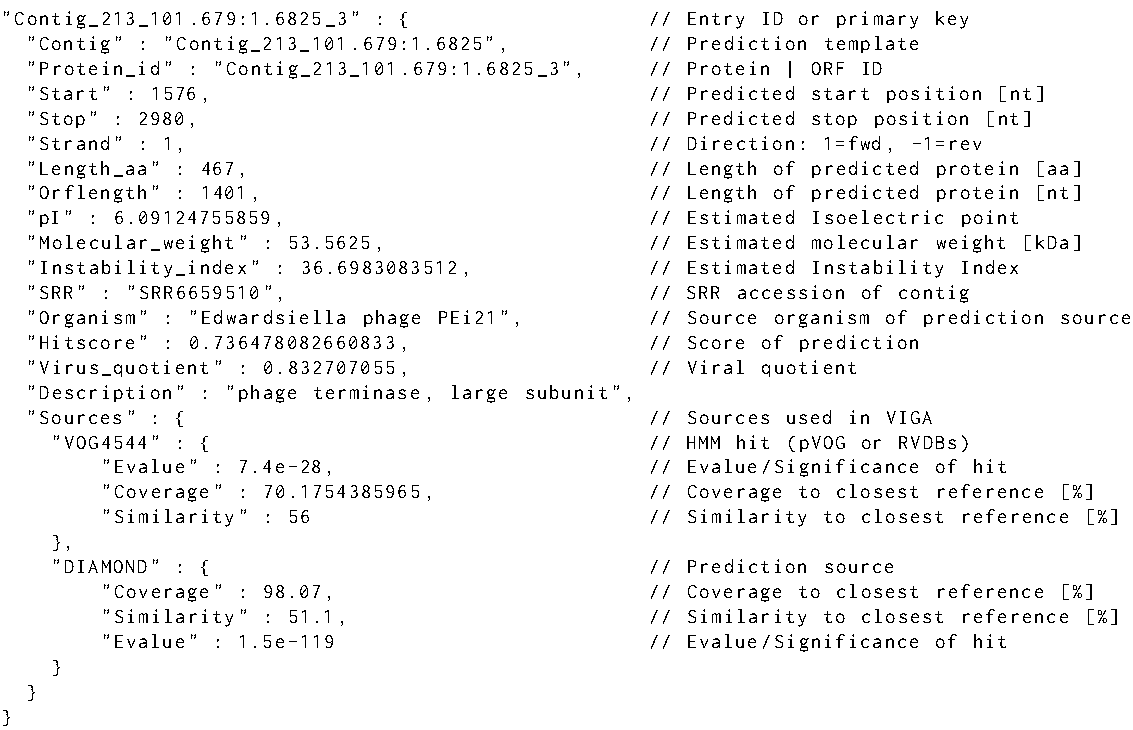
\includegraphics[width=0.6\textwidth]{figs/viga_json.pdf}
    \caption{Example of annotated  domain output in JSON format.
            \label{fig:sm_dm_outp}}
  \end{figure}

\section{Machine Learning Methods}
  \label{sec:sm_ml}
  Jaccard distance was estimated on the identified viral contigs using MASH
  \cite{Ondov2019}. MASH provides the user with a rapid method to reduce DNA sequences in
  representative k-mer sketches that are used to estimate a Jaccard similarity
  between samples. The tool was shown to be scalable in both number of
  considered metagenomes and size of the samples. MASH was shown to be a
  reliable tool to cluster amplicon datasets, metagenome read datasets and
  contig datasets \cite{Choi2018}.

  A kmer size of 21bp was chosen with a sketch size of 10,000. Samples
  containing less than two viral contigs were removed from the analysis.
  A total of 511 samples were kept for the analyzed and clustered by ward
  clustering. A manual cleaning of the terms was performed to remove
  punctuation and low-informative terms. In total, 210 samples with abstract
  and comments were analyzed.

\section{Index Methods}
  \label{sec:sm_idx}
  Setting up test data and databases: Three virtual machines were setup with
  Solr, MongoDb and PostgreSQL. Test tables were created through running a
  bigquery generate test tables with n entries to test the three databases. To
  generate these tables, we used a script saved in GitHub at:
  \url{https://github.com/NCBI-Hackathons/VirusDiscoveryProject/blob/master/ScalableIndex}.
  Three test tables were generated with 100 entries, and one million entries
  for SRA metadata, contig description and known contigs metadata. This was
  done without optimization or indexing.

  Uploading test data to the database: To upload the data to Solr, we used a
  schemaless document upload with the Solr interface. A script was used to
  import the JSON files to MongoDB (uploaded to GitHub), and another script was
  written to upload the data to PostgreSQL. PostgreSQL was the only database
  where the data types for each field needs to be defined. Overall, the data
  import for all three databases took less than a minute for the different
  databases and the test datasets generated.

  Indexing the field: Solr indexes all the fields in the document when uploaded
  as a schemless import. No fields were indexed for MongoDB and PostgreSQL with
  the current setup and files. This could have serious performance
  consequences, as the lookup complexity for non-indexed sql is usually
  considered on the order of n, where n is the number of elements in the
  database. For searching where an indexed field is used as the primary clause,
  the complexity is $n * log(n)$.












\end{document}
